\documentclass[conference]{IEEEtran}
\usepackage[ruled,vlined]{algorithm2e}
\usepackage{amsmath}
\usepackage[english]{babel} %localisation
\usepackage{caption,subcaption} %supposedly incompatible with Springer and IOP, IEEETran and ACM SIG
\usepackage{cite} %nice citations, e.g. [1--5]
\usepackage{fixltx2e} %fix latex bugs
\usepackage{graphicx}
\PassOptionsToPackage{hyphens}{url}\usepackage{hyperref} %clickable URLS
\usepackage[htt]{hyphenat} %hyphenate \texttt
\usepackage{microtype} %makes text pretty; also condenses
\usepackage{multirow} %multiple rows in tables
\usepackage{siunitx,textcomp} %\SI{value}{unit}, \si{unit}; textcomp for microtype compatibility
%\usepackage [caption=false]{subfig} %if caption/subcaption not available
% \usepackage{tikz,pgfplots} %drawings and plots
\usepackage[siunitx]{circuitikz} %circuit figures
\usepackage[T1]{fontenc} %ensure proper hyphenation and treatment of math in sentences
\usepackage{booktabs}
\bibliographystyle{IEEEtran}

\usepackage{tikz}
\usepackage{verbatim}
\usepackage{listings}
\begin{document}
\lstset{defaultdialect=[x86]{Assembler}}

% paper title
% can use linebreaks \\ within to get better formatting as desired
\title{Side Channel Analysis of an Embedded/Hardware Crypto Device}

% author names and affiliations
% use a multiple column layout for up to three different
% affiliations
\author{\IEEEauthorblockN{Sam Mitchell and Nathanael Weidler}
\IEEEauthorblockA{Deptartment of Electrical and Computer Engineering\\
Utah Stat University\\
Logan, Utah 84322\\
e-mail: samuel.alan.mitchell@gmail.com, NWeidler@gmail.com}
}

% make the title area
\maketitle


\begin{abstract}
%\boldmath
% Summarize project and results (executive summary).
%
This paper describes a side channel analysis attack on a microprocessor.  The microprocessor is running a Data Encryption Standard (DES) algorithm.  The goal of the attack is to recover the secret key from the device.  This is done by capturing the power usage of the device and using differential power analysis to analyze the data. 
 
\end{abstract}

\begin{IEEEkeywords}
Data Encryption Standard, Differential Power Analysis, Security.
\end{IEEEkeywords}

\section{Introduction}
	Side channel analysis is one way to attack even the most computationally complex cryptographic devices.  Through side channel analysis, information (such as secret keys) can be obtained from devices without using more traditional or brute force attacks.  In order to carry out a side channel analysis attack, the attacker must have access to the device.  The attacker then obtains power information using an oscilloscope connected to a resistor put in series with the device's power input.

	In this paper a side channel analysis will be carried out on an Tiva-C  microprocessor to obtain the secret key from a Data Encryption Standard (DES) algorithm.  First, a typical DES implementation was written and loaded into the flash of the Tiva-C microprocessor.  Next, the side channel analysis was carried out.  After the power information, or traces, were obtained, a technique called differential power analysis (DPA) was used to analyze the data.  \cite{des} \cite{Messerges}


\subsection{Structure of paper}
	The organization is as follows: in Section \ref{sec::des_impl}, the development of the DES implementation is presented.  In Section \ref{sec::expr} the experimental test setup for the capturing of the traces is described. Section \ref{sec::analysis} contains the analysis of the data.  Conclusions are detailed in Section \ref{sec::conclusion}. 


\section{DES Implementation} \label{sec::des_impl}
	As a part of this work an implementation of DES was written for the Tiva-C microprocessor.  "The DES Algorith Illustrated" was a valuable resource during this process.  All of the explicit details of DES will be left to other work, however, a brief overview will be presented in order for the reader to grasp the complexity of the algorithm. \cite{des}

	DES is a 16 round encryption algorithm.  It works on 64-bit blocks of plaintext and outputs encrypted data of the same size.  The output of the algorithm is the cipher text.  The first step in DES is to divide the plaintext block in half, the left 32-bits and the right 32-bits.  The heart of DES is the 56-bit master key which is used to create 16 distinct 48-bit round keys, one for each round of the algorithm.  (The intent of this attack is to recover the key from the 16th round, from which all other keys can be easily obtained.)  To create each round key the 56-bit key is permuted and divided into two halves.  Then for each round each of those halves is shifted, recombined and permuted yielding the 48-bit round keys.

	One half of the plaintext (32-bits) is expanded and permuted to create a 48-bit word which is xored with the round key.  The result is divided into eight 6-bit parts which go through 8 distinct s-boxes.  An s-box is  method to substitute a 6-bit input with a 4-bit output.  These 4-bit outputs are put back together and permuted to create a 32-bit word which is xored with the other half of the plaintext.  This process is repeated 16 times until finally the two halves are put back together and permuted one last time to create the cipher text.  An illustration of one round is shown in figure \ref{fig:round}.

	\begin{figure}[h]
	\centering
	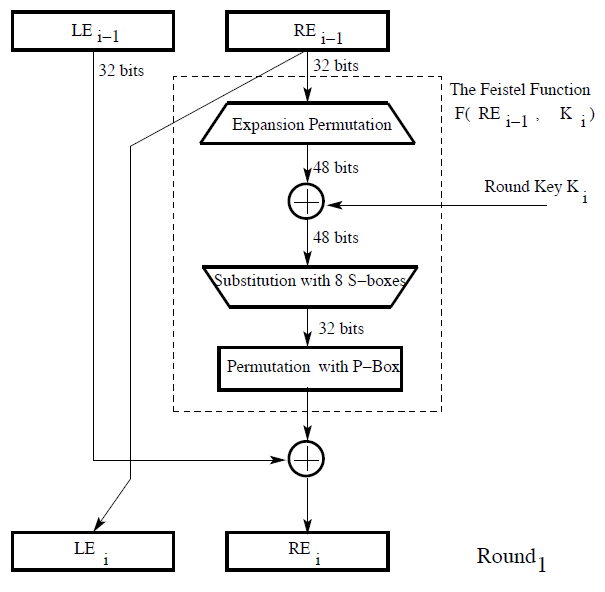
\includegraphics[width=0.7\linewidth]{./round}
	\caption{One round of DES.}
	\label{fig:round}
	\end{figure}




\subsection{DES Modifications}
	In order to facilitate the process by which traces are obtained, there was an addition to the traditional DES algorithm.  This slight modification in no way compromises the integrity of the algorithm or its outputs.  The change was to hold a general purpose input/output (GPIO) high during the algorithm except during a single instruction in which the output of the Feistel function is xored with the other half of the plaintext in round 16 and the result is written back to a register.  This allowed an oscilloscope to be triggered on the falling edge of the GPIO and frame this critical step which will be discussed later.  There were also two no-operations (nops) added before this register write and one after to allow the GPIO to settle and facilitate a cleaner capture.  The output of the assembly dump with comments added can be seen in figure \ref{fig:asm_snippet}.
	
	\begin{figure}[h]
	\centering
	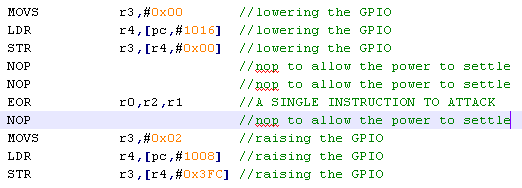
\includegraphics[width=0.7\linewidth]{./asm_snippet}
	\caption{The assembly showing the GPIO writes surrounding the xor and register write under attack.}
	\label{fig:asm_snippet}
	\end{figure}

	

\section{Experimental Setup} \label{sec::expr}
	This portion of the experiment was the most crucial to its success.  The goal is to obtain information about the power usage of the microprocessor during a critical step of the DES algorithm.  During a register write operation the power used will be different depending on the value of the word written.  It is believed that by analyzing this information, the secret key to the algorithm can be obtained.
	
	The oscilloscope used was a Techtronix ??? the sample rate was 1 giga-sample per second and each trace contained about 650 samples.
	
	The setup used involved the Tiva-C microprocessor powered by a bench top power supply through a breadboard.  The ground connection between the microprocessor and the power supply had a 1-ohm resistor added in series.  An Oscilloscope probe was placed on the resistor so that the voltage could be measured.  Then another oscilloscope probe was placed on the GPIO pin discussed in the previous section to act as the trigger.  The voltage data would be taken twenty times for each plain text value used in the DES algorithm and then averaged in an attempt to reduce noise.  91,840 captures with 4,592 unique plain text values would be obtained.  Each trace takes about two seconds to capture so the time to obtain all traces is 183,680 seconds or about 51 hours, or 2.13 days.  The voltage data acquired would be analyzed later to determine the secret key.
	
	The test setup needed to be automated to facilitate the capturing of the traces.  In order for this to be done a matlab file was written to interface with the oscilloscope.  As trivial as this may sound it was not easy.  It took many hours of learning the oscilloscope and the commands to control it through matlab.  It also took time and patience to fine tune the DES implementation to create enough delay between each run of the algorithm to allow for the oscilloscope to transfer the data capture and re-arm itself.
	

\section{Analysis of the Data}\label{sec::analysis} 
	In order to analyze the data, differential power analysis (DPA) was employed.  Round 16 was chosen for this because given the cipher text, the input to the Feistel  function and the output from the second xor (seen in the bottom right of figure \ref{fig:round}) can be determined.  Then the round key is guessed six bits at a time.  This greatly reduces the complexity of the key as there are only 64 possible combinations for a guess of six bits of the key.  Using knowledge of the Feistel function and the six bit key guess, the output of the Feistel function can be guessed at four bits at a time.  Remember, the s-boxes reduce the data from 48 bits to 32 bits.  This output is xored with the D value, and we already know the output of this xor.  So guessing one input and knowing the output determines the other input to the xor gate.  
	
	For each key guess four bits of the D word are deduced.  These 4-bit groups are divided into 3 sets where set 0 contains all guesses for which the four bits guessed are "0000," set 1 contains all guess where the four bits are "1111," and set 2 contains all other guessed values.  The average power for each sample point for sets 0 and 1 is calculated.  The two average powers are subtracted from each other.  The correct key guess will show large spikes where the calculation was actually made on the trace.  This process is repeated eight times, once for each s-box until the correct key is determined.
	

\section{Results}\label{res}

\section{Conclusion}\label{sec::conclusion} 


% Summarize results and lessons learned.
	% This paper considers the efficient computation of passwords. Multiple methods to increase hashing throughput are presented. It is shown that hardware implementation of a password cracker provides more throughput per unit dollar than a software implementation. Future research will address the efficacy of different architectures in password computation. 
	As can be seen, side channel analysis can be an effective means to recover data from embedded systems.  DPA has previously been shown to work.  It seems the determining factor of whether or not your side channel analysis will be a success is the acquisition of the.
\bibliography{report}
% that's all folks




\end{document}